\documentclass[12pt,letterpaper]{article}

\usepackage{common}
\usepackage{amsmath,amsfonts,amssymb,bbm}
\usepackage{palatino}
\usepackage[linkcolor=blue]{hyperref}
\usepackage{fullpage}
\usepackage{color}
\usepackage{enumitem}
\usepackage{titlesec}
\usepackage[textsize=tiny]{todonotes}
\hypersetup{
    colorlinks=true,
    linkcolor=blue,
    filecolor=magenta,
    urlcolor=cyan,
}
\newcommand{\TODO}[1]{\todo[inline]{#1}}
\newcommand{\R}{\mathbbm{R}}
\newcommand{\mba}{\mathbf{a}}
\newcommand{\mbb}{\mathbf{b}}
\newcommand{\boldphi}{\boldsymbol{\phi}}
\newcommand{\mbx}{\mathbf{x}}
\newcommand{\mbxt}{\tilde{\mathbf{x}}}
\newcommand{\Sigmat}{\tilde{\Sigma}}
\newcommand{\mbz}{\mathbf{z}}
\newcommand{\mbw}{\mathbf{w}}
\newcommand{\eps}{\epsilon}
\newcommand{\Ut}{\tilde{U}}
\newcommand{\angstrom}{\textup{\AA}}
\newcommand{\E}{\mathrm{E}}
\newcommand{\Var}{\mathrm{Var}}
\newcommand{\p}{\partial}

\newcommand{\false}{{\it false}}
\newcommand{\true}{{\it true}}
\newcommand{\nutr}{{\it nutr}}
\newcommand{\pois}{{\it pois}}


\begin{document}
\begin{center}
    CS 181 Spring 2019 Section 3 Notes \textbf{SOLUTIONS}\\
(Bayesian Approaches, Gradient Descent, Linear Classification)\\
\href{https://colab.research.google.com/drive/1AJRaGeqgTosVNWjinYPahB1RHGAOwIh-}{Interactive Demo}
\end{center}



\section{Bayesian Linear Regression}

\subsection{Parameter Distributions}

Let $D = \{(\mathbf{x}_i, y_i)\}_{i=1}^n$, $\mathbf{x}_i \in \mathbb{R}^m$, $y_i \in \mathbb{R}$. Consider the generative model:

\begin{align}
y_i \sim \mathcal{N}(\mathbf{w}^\top \mathbf{x}_i, \beta^{-1})
\end{align}
\noindent The likelihood of the data has the form:

\begin{align}
    p(\mathbf{y}|\mathbf{X},\mathbf{w}) = \mathcal{N}(\mathbf{y}|\mathbf{X}\mathbf{w},\beta^{-1}\mathbf{I})
\end{align}
\noindent Put a conjugate prior on the weights (assume precision $\beta^{-1}$ known):

\begin{align}
    p(\mathbf{w}) = \mathcal{N}(\mathbf{w}|\mathbf{m}_0, \mathbf{S}_0)
\end{align}
\noindent We want a posterior distribution on $\mathbf{w}$. Using Bayes' Theorem:

\begin{align}
    p(\mathbf{w}|D) \propto p(D|\mathbf{w})p(\mathbf{w})
\end{align}
\noindent It turns out that our posterior after $n$ examples is also Gaussian:

\begin{align}
    p(\mathbf{w}|D) = \mathcal{N}(\mathbf{w}|\mathbf{m}_n, \mathbf{S}_n)
\end{align}
where
\begin{align}
    \mathbf{S}_n &= \left(\mathbf{S}_0^{-1} + \beta \mathbf{X}^\top\mathbf{X}\right)^{-1}\\
    \mathbf{m}_n &= \mathbf{S}_n(\mathbf{S}_0^{-1}\mathbf{m}_0 + \beta \mathbf{X}^\top\mathbf{y})
\end{align}

\subsection{Posterior Predictive Distributions}

We have seen how to obtain a posterior distribution over $\mathbf{w}$. But, given this posterior and a new data point $\mathbf{x}^{*}$,
how do we actually make a prediction $y^{*}$? How do we deal with \textit{uncertainty} about $\mathbf{w}$? Consider this:
\begin{align}
p(y^{*}| \mathbf{x}^{*}, \mathcal{D}) &= \int_{\mathbf{w}} p(y^{*}|\mathbf{x}^{*}, \mathbf{w})p(\mathbf{w} | \mathcal{D}) d\mathbf{w}\\
&= \int_{\mathbf{w}} \mathcal{N}(y^{*}|\mathbf{w}^\top\mathbf{x}^{*}, \beta^{-1}) \mathcal{N}(\mathbf{w}|\mathbf{m}_n, \mathbf{S}_n) d\mathbf{w} 
\end{align}

\noindent This is the \textbf{posterior predictive} distribution over $y^{*}$. This can be interpreted as a weighted average of many predictors, 
one for each choice of $\mathbf{w}$, weighted by how likely $\mathbf{w}$ is according to the posterior. Since each of the terms on the right hand side 
follows a normal distribution, we can use some math (see CS181 2017 lecture 5, slide 33) to find that:
\begin{align}
p(y^{*}| \mathbf{x}^{*}, \mathcal{D}) = \mathcal{N}(y^{*}| \mathbf{x}^{*\top}\mathbf{m}_n, \mathbf{x}^{*\top}\mathbf{S}_n\mathbf{x}^{*} + \beta^{-1})
\end{align}

\section{Gradient Descent}
Gradient descent is an iterative algorithm for finding the minimum of a function. 

\subsection{Gradient vector}
If $f$ is a scalar-valued, its derivative is a column vector we call the gradient vector.
\begin{align}\frac{d f(\boldx)}{d\boldx} =\begin{pmatrix}\frac{\partial f(\boldx)}{\partial x_1} \\ \frac{\partial f(\boldx)}{\partial x_2}\\ \dots \\ \frac{\partial f(\boldx)}{\partial x_n}\end{pmatrix}\end{align}
The gradient vector points in the direction of steepest ascent in $f(\boldx)$. This is useful for optimization.

\subsection{Gradient Descent Algorithm}
If we want to find the value of a vector $\boldw$ that minimizes a function $f(\boldw)$, we start with an initial guess $\boldw^{(0)}$ and at each time step $i$ we update our guess by going in the direction of the greatest descent (opposite the direction of the gradient vector).
\begin{align}
\boldw^{(i+1)} = \boldw^{(i)} - \eta \frac{d f(\boldw^{(i)})}{d\boldw^{(i)}}\end{align}
where $\eta > 0$ is known as the learning rate.

See this \href{https://colab.research.google.com/drive/1AJRaGeqgTosVNWjinYPahB1RHGAOwIh-}{notebook} for an interactive demo of gradient descent with visualizations. \\
\textbf{Note: } The notebook also has information about one-hot encodings.

\subsection{Stocastic Gradient Descent}
This method makes an update to the weight vector based on one data point at a time. 

The algorithm is as follows:
\begin{enumerate}
    \item Sample data point i, corresponding to $(\boldx_i,y_i)$\\
    This is done by cycling through the data either in sequence or by selecting points at random with replacement.
    \item Compute loss and gradient for for just that data point
    \item Update $\boldw$ based on this stochastic gradient.
\end{enumerate}

\section{Classification}
The goal in classification is to take an input vector $\mathbf{x}$ and assign it to one of $K$ discrete classes $C_k$, where $k = 1, \hdots, K$.
The input space is thus divided into \textbf{decision regions} whose boundaries are called \textbf{decision boundaries or surfaces}.

\subsection{Binary Linear Classification}

A discriminant function is one that directly assigns each vector $\mathbf{x}$ to a specific class. We first assume two classes, i.e. our responses are binary and $K=2$. Linear classification seeks to divide the 2 classes by a linear separator in the feature space: 
if $m=2$, the separator is a line; if $m=3$, the separator is a plane; for general $m$, the separator is a $(m-1)$-dimensional hyperplane.
The simplest representation of a linear discriminant function is obtained by taking a linear function of the input vector as such:
\begin{align}
h(\mathbf{x};\mathbf{w}, w_0) = \mathbf{w}^\top\mathbf{x} + w_0
\end{align}
\noindent The corresponding decision boundary is defined by the relation $h(\mathbf{x};\mathbf{w},w_0) = 0$.
The classifier will predict $\hat{y}=1$ if
$h(\mathbf{x};\mathbf{w},w_0)>0$, and predict $\hat{y}=-1$ otherwise.\\

\noindent Weight vector $\mathbf{w}$ is orthogonal to every vector lying within the decision surface, 
and so $\mathbf{w}$ determines the orientation of the decision boundary. Remember the familiar
plane equations $c_1x + c_2y + c_3z + c_4 = 0$ for fixed constants $\mathbf{c}$ and variables $x,y,z$? 
These are just dot products with an orthogonality constraint, and thus, they are precisely the kinds of boundaries described here.
%By definition, the normalized distance from the origin to a point
%$\mathbf{x}$ on the boundary is $\frac{\mathbf{w}^\top\mathbf{x}}{\|\mathbf{w}\|}$. 
%Noting that $h(\mathbf{x};\mathbf{w},w_0)=\mathbf{w}^\top \mathbf{x}+w_0=0$,
%since $\mathbf{x}$ is on the decision boundary, we substitute 
%$\mathbf{w}^\top\mathbf{x}=-w_0$ to get
%
%$$\frac{\mathbf{w}^\top\mathbf{x}}{\|\mathbf{w}\|} = - \frac{w_0}{\|\mathbf{w}\|},$$
%
%and see that $w_0$ together with $\|\mathbf{w}\|$ define the location
%of the decision boundary where $w_0$ is a bias/offset term. 
The input space can also be transformed through a (potentially non-linear) basis function:
$h(\mathbf{x};\mathbf{w},w_0)=\mathbf{w}^\top\boldsymbol{\phi}(\mathbf{x})+w_0,$.
This can help with linear separability. More on this soon with neural networks.

\subsection{Perceptron Algorithm}

An important way to train a linear discriminant model is via the perceptron algorithm. 
This works for a two-class model. Rather than a 0/1 error function (or sum-squared error), 
the perceptron algorithm adopts an alternative error function known as hinge loss, which uses
the following function :
\begin{align}
    ReLU(z) &= \begin{cases}
      z & z > 0\\
      0 & o.w. 
    \end{cases} = \max\{0, z\}	
\end{align} 

\noindent called a rectified linear activation (ReLU). This function is useful in the following way. Since $h()>0$ for $y=1$ and $h()<0$ for $y=-1$,
the product $-h(\mathbf{x}_i;\mathbf{w},w_0) y_i>0$ when there is a classification error.
The perceptron loss function is defined as:
\begin{eqnarray}
   \mathcal{L}(\mathbf{w}) &=&  \sum_{i=1}^n ReLU(-h(\mathbf{x}_i;\mathbf{w},w_0) y_i)  \\
    &=&  -\sum_{i=1:y_i \neq \hat{y}_i}^n (\mathbf{w}^\top\mathbf{x}_i + w_0) y_i
\end{eqnarray}

\noindent 
The first term takes the sum over all training examples of the ReLU function
applied to $-h(\mathbf{x}_i;\mathbf{w},w_0) y_i$. When 
there is a misclassified example, then this value is positive
and it counts as a loss. 
Equivalently, we can simply write this as the 
negated sum over all misclassified examples 
of $h(\mathbf{x}_i;\mathbf{w},w_0) y_i$.

This loss function has a gradient that is easier to work with than if we had used a 0/1 error function, and we can now apply stochastic gradient descent. 
%
The change in weight vector from step $t$ to $t+1$ is given by the following
iteration on an incorrect example:
%
\begin{align}
\mathbf{w}^{(t+1)} = \mathbf{w}^{(t)} - \eta \frac{\partial}{\partial \mathbf{w}} \mathcal{L}^{(i)}(\mathbf{w}) = \mathbf{w}^{(t)} + \eta y_i\mathbf{x}_i,
\end{align}
%
\noindent
where $\eta$ is the learning rate parameter. Note that as the weight vector evolves during training, the set of examples that are misclassified will also change.

\newpage

\section{Practice Questions}

\begin{enumerate}

\item {\bf Posterior Weight Distribution By Completing the Square (Bishop 3.7)}\\
\fbox{\parbox{\linewidth}{%

        We know from (3.10) in Bishop that the likelihood can be written as 

\begin{align*}
p(\mathbf{y} | \mathbf{X}, \mathbf{w}) &= \prod_{i=1}^n \mathcal{N}(y_i | \mathbf{w}^\top \mathbf{x}_i, \beta^{-1}) \\
&\propto \exp \left( -\frac{\beta}{2} (\mathbf{y} - \mathbf{X}\mathbf{w})^\top (\mathbf{y} - \mathbf{X}\mathbf{w}) \right)
\end{align*}



where precision $\beta = \frac{1}{\sigma^2}$ and in the second line above we have ignored the Gaussian normalization constants. 
By completing the square, show that with a prior distribution on $\mathbf{w}$ given by $p(\mathbf{w}) = \mcN(\mathbf{w} | \mathbf{m}_0,\mathbf{S}_0)$, 
the posterior distribution $p(\mathbf{w} | D)$ is given by 
\begin{align*}
p(\mathbf{w} | D) = \mcN(\mathbf{w} | \mathbf{m}_n, \mathbf{S}_n)
\end{align*}
where
\begin{align*}
\mathbf{m}_n &= \mathbf{S}_n(\mathbf{S}_0^{-1}\mathbf{m}_0 + \beta \mathbf{X}^\top \mathbf{y}) \\
\mathbf{S}_n &= \left(\mathbf{S}_0^{-1} + \beta \mathbf{X}^\top \mathbf{X}\right)^{-1}
\end{align*}

Here's the first step. Take ln[(likelihood)(prior)] and collect normalization terms that don't depend on $\mathbf{w}$:
\begin{align*}
\ln p(\mathbf{w} | D) &\propto \ln p(\mathbf{y} |\mathbf{X}, \mathbf{w}) +\ln p(\mathbf{w}) \\
&=\mathit{const} -\frac{\beta}{2} (\mathbf{y} - \mathbf{X} \mathbf{w})^\top (\mathbf{y} - \mathbf{X} \mathbf{w})  -\frac{1}{2} (\mathbf{w} - \mathbf{m}_0)^\top \mathbf{S}_0^{-1} (\mathbf{w} - \mathbf{m}_0)
\end{align*}

Hint: Remember, you already know what the posterior should look like.
Once you simplify your expression enough, try foiling the posterior in terms of
$\mathbf{m}_n$ and $\mathbf{S}_n^{-1}$ and see if you can see the relationship
between your expression and this posterior.
}}


\newpage

\textbf{Solution:}

As the problem statement suggestions, the first step is to take ln[(likelihood)(prior)] and collect normalization terms that don't depend on $\mathbf{w}$:
\begin{align}
\ln p(\mathbf{w} | D) &\propto \ln p(\mathbf{y} |\mathbf{X}, \mathbf{w}) +\ln p(\mathbf{w}) \\
&=\mathit{const} -\frac{\beta}{2} (\mathbf{y} - \mathbf{X} \mathbf{w})^\top (\mathbf{y} - \mathbf{X} \mathbf{w})  -\frac{1}{2} (\mathbf{w} - \mathbf{m}_0)^\top \mathbf{S}_0^{-1} (\mathbf{w} - \mathbf{m}_0)
\end{align}

Expanding, we have:
%
\begin{align}
\mathit{const} -\frac{1}{2}\left( \beta \mathbf{y}^\top \mathbf{y} - \beta \mathbf{y}^\top\mathbf{Xw}
- \beta\mathbf{w}^\top\mathbf{X}^\top\mathbf{y} + \beta\mathbf{w}^\top\mathbf{X}^\top \mathbf{Xw} \right)\\
+ \left( \mathbf{w}^\top \mathbf{S}_0^{-1}\mathbf{w} - \mathbf{w}^\top \mathbf{S}_0^{-1}\mathbf{m}_0 - \mathbf{m}_0^\top \mathbf{S}_0^{-1}\mathbf{w} + \mathbf{m}_0^\top \mathbf{S}_0^{-1}\mathbf{m}_0 \right)
\end{align}



Important: Remember that terms like $\mathbf{y}^\top\mathbf{Xw}$ are the same scalar as $\mathbf{w}^\top\mathbf{X}^\top\mathbf{y}$.
Collecting together quadratic and linear terms, factoring the $\mathbf{w}$s out, and moving terms that
don't depend on $\mathbf{w}$ into the constant, we have
%
\begin{align}
\mathit{const}-\frac{1}{2}\left( \mathbf{w}^\top(\mathbf{S}_0^{-1} + \beta \mathbf{X}^\top \mathbf{X}) \mathbf{w} 
-2\mathbf{w}^\top (\mathbf{S}_0^{-1}\mathbf{m}_0 + \beta \mathbf{X}^\top \mathbf{y}) \right)
\end{align}

Put aside what we have done so far. Recall that our target looks like:
\begin{align}
-\frac{1}{2}\left((\mathbf{w} - \mathbf{m}_n)^\top \mathbf{S}_n^{-1} (\mathbf{w} - \mathbf{m}_n) \right),
\end{align}
When expanded, this looks like
\begin{align}
-\frac{1}{2}\big(\mathbf{w}^\top \mathbf{S}_n^{-1}\mathbf{w} -
                  \mathbf{m}_n^\top\mathbf{S}_n^{-1}\mathbf{w} -
                  \mathbf{w}^\top\mathbf{S}_n^{-1}\mathbf{m}_n +
                  \mathbf{m}_n^\top\mathbf{S}_n^{-1}\mathbf{m}_n
               \big)
\end{align}
Drop the term that doesn't have $\mathbf{w}$ and combine the two middle terms
\begin{align}
-\frac{1}{2}\big(\mathbf{w}^\top \mathbf{S}_n^{-1}\mathbf{w} -
                   2\mathbf{w}^\top\mathbf{S}_n^{-1}\mathbf{m}_n
                \big)
\end{align}
This looks like what we ended up with in (20) where 
$$
\mathbf{S}_n^{-1} = \mathbf{S}_0^{-1} + \beta \mathbf{X}^\top \mathbf{X}
$$
and
%
$$
\mathbf{S}_n^{-1}\mathbf{m}_n = \mathbf{S}_0^{-1}\mathbf{m}_0 + \beta \mathbf{X}^\top \mathbf{y},
$$
%
as required.
%
This has the desired form of an (unnormalized) Gaussian.

\newpage

\item {\bf Properties of Softmax }\\
\fbox{\parbox{\linewidth}{



Consider a $K$-class classification problem.
Let $\{\boldw_k\}_{k=1}^K$ be defined such that for some data 
point $\mathbf{x}$, $z_k = \mathbf{w}_k^\top\mathbf{x}$ can be interpretted as a 
score for $\mathbf{x}$ belonging to class $k$. Multi-class Logistic Regression (LR) with a trained 
set of weights assigns $\mathbf{x}$ the class $k$ for which
it has the highest such score. The \textbf{softmax transformation} takes as input a vector, and
outputs a transformed vector of the same size.

\[ \mathrm{softmax}(\boldz)_k =\frac{\exp(z_k)}{\sum_{\ell=1}^K \exp(z_{\ell})}, \ \ \text{for all $k$}\]

LR uses the softmax over a vector of $K$ scores
$\mathbf{z} = [\boldw_1^\top\mathbf{x}, \ldots, \boldw_K^\top\mathbf{x}]$ so that it can be normalized
and intepretted as a vector of \textit{probabilities}.
  \begin{align*}
    p(\boldy=C_k \given \boldx; \{\boldw_{\ell}\}_{\ell=1}^K)
    &= \mathrm{softmax}([\boldw_1^{\top}\boldx \ldots \boldw_K^{\top} \boldx]^\top)_k =  \frac{ \exp( \boldw_k^{\top}\boldx ) }
    {  \sum_{\ell=1}^K \exp( \boldw_{\ell}^{\top}\boldx ) }\,.
  \end{align*}

\noindent where $C_k$ is a \textit{one-hot} vector with a $1$ in coordinate $k$ and $0$s elsewhere.

  Assuming data $D = \{(\boldx_i, \boldy_i)\}_{i=1}^N$,
  the negative log-likelihood can be written as:

  \[\mcL(\{\boldw_{\ell}\}) = - \sum_{i=1}^N \ln p(\boldy_i \given \boldx_i; \{\boldw_{\ell}\}) \]

  The softmax is an important function and you will see it again in other models, such as neural networks.
  In this problem, we aim to gain intuitions into the properties of
  softmax and multiclass logistic regression. In the section note solutions,
  we provide arguments for facts (a), (b), (c), and (d) (make sure you verify
  these on your own time). Using (d), show that (e) holds:\\

  \begin{enumerate}
      \item The output of the softmax is a vector with non-negative components
      that are at most 1. 

      \item The output of the softmax defines a distribution, so the components sum to 1.

      \item Softmax preserves order. This means that if elements $z_k < z_\ell$
    in $\boldz$, then  $\mathrm{softmax}(\boldz)_k < \mathrm{softmax}(\boldz)_{\ell}$ for any $k,\ell$. 
      \item \[\frac{\partial \mathrm{softmax}(\boldz)_k }{\partial z_j} = \mathrm{softmax}(\boldz)_k (I_{kj} - \mathrm{softmax}(\boldz)_j) \ \ \text{for\ any\ } k, j  \]

    where indicator $I_{kj}=1$ if $k=j$ and $I_{kj}=0$ otherwise.

    \item Using (d), show that:
       \[ \frac{\partial }{\partial \boldw_j} \mcL(\{\boldw_{\ell}\}) = \sum_{i=1}^N 
       \big[p(\boldy_i = C_j | \boldx_i; \{\boldw_\ell\}) - y_{ij} \big] \boldx_i  \]
    
  \end{enumerate}
}}

  \newpage

  \textbf{Solution:}

    % Solution
        \begin{enumerate}
            
            \item  The $j^{th}$ component of the softmax function $\text{softmax}({\bf z})$ is:
            \[\text{softmax}({\bf z})_j = \frac{\exp(z_j)}{\sum_i \exp(z_i)}.\]
            
            As $\exp(x)>0$ for all $x\in\mathbb R$, we have $\exp(z_j)>0$ and $\sum_i \exp(z_i)>0$. Thus the output of the softmax function is a vector with non-negative components. Since $\exp(z_j)$ appears in both the numerator and the denominator (as the $i=j$ term in the sum), the denominator must be at least as large as the numerator, and so the components are at most 1.
            
            
            \item  Summing over the components:
            \[\sum_j \text{softmax}({\bf z})_j = \sum_j \frac{\exp(z_j)}{\sum_i \exp(z_i)} =  \frac{\sum_j\exp(z_j)}{\sum_i \exp(z_i)}  = 1.\]

            
            \item If $z_j\ge z_k$, then $\exp(z_j)\ge \exp(z_k)$ as the exponential is a monotonically increasing function. Dividing by the positive constant $\sum_i \exp(z_i)$, this inequality implies that:
            \[\text{softmax}({\bf z})_j = \frac{\exp(z_j)}{\sum_i \exp(z_i)} \ge \frac{\exp(z_k)}{\sum_i \exp(z_i)} = \text{softmax}({\bf z})_k,\]
            which shows that the softmax function preserves the order of the elements of ${\bf z}$.
            
  
          
            \item To relate our notation to Bishop (4.106), note that $y_k = \text{softmax}({\bf z})_k$ and $a_j = z_j$. 
            
            If $j\neq k$, then:
            \begin{align*}
            \frac{\partial \text{softmax}({\bf z})_k}{\partial z_j} &= \frac{\partial}{\partial z_j} \frac{\exp(z_k)}{\sum_i \exp(z_i)} = - \frac{\exp(z_k)}{\left(\sum_i \exp(z_i)\right)^2}\exp(z_j)\\& = -\frac{\exp(z_k)}{\sum_i \exp(z_i)} \frac{\exp(z_j)}{\sum_i \exp(z_i)} = -\text{softmax}({\bf z})_k \text{softmax}({\bf z})_j.
            \end{align*}
            
            If $j = k$ then:
            \begin{align*}
            \frac{\partial \text{softmax}({\bf z})_k}{\partial z_j} &= \frac{\partial}{\partial z_j} \frac{\exp(z_k)}{\sum_i \exp(z_i)} = \frac{\exp(z_k)}{\sum_i \exp(z_i)} - \frac{\exp(z_j)^2}{\left(\sum_i \exp(z_i)\right)^2}  \\&= \left(1 - \frac{\exp(z_k)}{\sum_i \exp(z_i)}\right)\frac{\exp(z_k)}{\sum_i \exp(z_i)} = \text{softmax}({\bf z})_k(1 - \text{softmax}({\bf z})_j).
            \end{align*}
            
            Putting these results together:
            \boxed{\frac{\partial \text{softmax}(\mathbf{z})_k}{\partial z_j} = \text{softmax}(\mathbf{z})_k(I_{kj} - \text{softmax}({\mathbf{z}})_j)}
            
            
            \item  Write the negative log-likelihood.
            
            $$
            \mcL(\{\boldw_{\ell}\}) = -\sum_{i=1}^N\sum_{k=1}^K y_{ik} \ln p(\boldy = C_k | \boldx_i; \{\boldw_\ell\})
            $$
            $$\frac{\partial }{\partial \boldw_j} \mcL(\{\boldw_{\ell}\}) =-\sum_{i=1}^N\sum_{k=1}^K y_{ik}\frac{\partial }{\partial \boldw_j} \ln p(\boldy = C_k | \boldx_i; \{\boldw_\ell\})
            $$
            \noindent Using Derivative of log + chain rule
            $$=-\sum_{i=1}^N\sum_{k=1}^K y_{ik}\bigg(\frac{1}{p(\boldy = C_k | \boldx_i; \{\boldw_\ell\})}\bigg)\frac{\partial }{\partial \boldw_j}p(\boldy = C_k | \boldx_i; \{\boldw_\ell\})$$
            \noindent Rewrite using chain rule
            $$ =-\sum_{i=1}^N\sum_{k=1}^K y_{ik}\bigg(\frac{1}{p(\boldy = C_k | \boldx_i; \{\boldw_\ell\})}\bigg)
               \frac{\partial }{\partial z_j} p(\boldy = C_k | \boldx_i; \{\boldw_\ell\}) \frac{\partial }{\partial \boldw_j} z_j$$
            The derivative at the end is just the derivative of a dot product:
            $$ =-\sum_{i=1}^N\sum_{k=1}^K y_{ik}\bigg(\frac{1}{p(\boldy = C_k | \boldx_i; \{\boldw_\ell\})}\bigg)
               \frac{\partial }{\partial z_j} p(\boldy = C_k | \boldx_i; \{\boldw_\ell\}) \mathbf{x}$$
            Use the derivative of the softmax found in (d)
            $$ = -\sum_{i=1}^N\sum_{k=1}^K y_{ik}\bigg(\frac{1}{p(\boldy = C_k | \boldx_i; \{\boldw_\ell\})}\bigg)
            \bigg(p(\boldy = C_k | \boldx_i; \{\boldw_\ell\})\bigg)\bigg(I_{kj} - p(\boldy = C_j | \boldx_i; \{\boldw_\ell\})\bigg) \mathbf{x}_i$$
            Notice that two terms are conveniently reciprocals and simplify
        $$= -\sum_{i=1}^N\sum_{k=1}^K y_{ik}\bigg(I_{kj} - p(\boldy = C_j | \boldx_i; \{\boldw_\ell\})\bigg)\mathbf{x}_i$$
        Foil the terms
        $$= -\sum_{i=1}^N\sum_{k=1}^K y_{ik}I_{kj}\mathbf{x}_i + \sum_{i=1}^N p(\boldy = C_j | \boldx_i; \{\boldw_\ell\})\mathbf{x}_i \bigg(\sum_{k=1}^C y_{ik}
        \bigg)$$
        The $I_{kj}$ in the first sum collapses the sum over $k$ to the term where $j=k$. As the $\mathbf{y}_{i}$ are \textit{one-hot}, 
        we have that $\sum_{k=1}^K y_{ik}=1$. Using these facts:
        $$ \frac{\partial }{\partial \boldw_j} \mcL(\{\boldw_{\ell}\}) = -\sum_{i=1}^N y_{ij}\mathbf{x}_i + \sum_{i=1}^N p(\boldy = C_j | \boldx_i; \{\boldw_\ell\})\mathbf{x}_i $$
        
        $$\boxed{ =
        \sum_{i=1}^N (p(\boldy = C_j | \boldx_i; \{\boldw_\ell\}) - y_{ij})\mathbf{x}_i}
        $$
        
       


        \end{enumerate}

\newpage

\item {\bf Small Perceptron Example }\\
\fbox{\parbox{\linewidth}{

Let's train a perceptron on a small data set. 
Consider data $\{\mathbf{x}_i\}_{i=1}^n, \mathbf{x}_i \in \reals^2$.
Let the learning rate $\eta = 0.2$ and let the weights be initialized as:
$$\mathbf{w} = \binom{w_1}{w_2} = \binom{1}{0.5}, w_0 = 0$$
Let the circles have $y_i=1$ and the triangles $y_i=-1$.
The data and initial separation boundary (determined by $\mathbf{w}$) is illustrated below.

\begin{center}
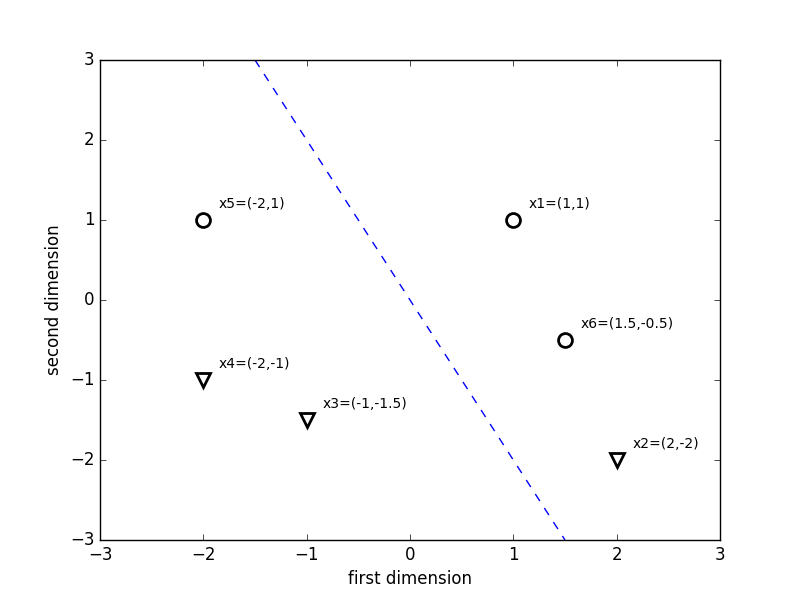
\includegraphics[width=0.8\textwidth]{perceptron.png}
\end{center}

Proceed by iterating over each example until there are no more classification errors. When in doubt, refer to the notes above.
We know a priori that we will be able to train the classifier and have no classification errors because one can see visually
that the data is linearly separable (note: as mentioned above, if the data were not so obviously linearly separable, a new basis
could make it so). How many updates do you have to make? Is this surprising?

}}


\newpage

\textbf{Solution:}

\begin{enumerate}
\item Consider $\mathbf{x_1}: \mathbf{w}^\top \mathbf{x_1} + w_0 = 1\cdot 1 + 0.5\cdot 1 + 0 > 0$. 
This is a correct classification, so we take no action.
\item Consider $\mathbf{x_2}: 
\mathbf{w}^\top \mathbf{x_2} + w_0 = 1\cdot 2 + 0.5 \cdot (-2) + 0 > 0$. 
This is an incorrect classification, so we need to update our weight parameters:
\begin{align*}
\mathbf{w} &\leftarrow \mathbf{w} + (0.2)(-1)\binom{2}{-2} = \binom{0.6}{0.9}\\
w_0 &\leftarrow w_0 + 0.2(-1) = -0.2
\end{align*}
\item Consider $\mathbf{x_3}: 
\mathbf{w}^\top \mathbf{x_3} + w_0 = 0.6 \cdot (-1) + 0.9 \cdot (-1.5) + (-0.2) < 0$. This is a correct classification.
\item Consider $\mathbf{x_4}:$ Check that this is a correct classification.
\item Consider $\mathbf{x_5}:$ Check that this is an incorrect classification 
and our weight parameters are updated to:
\begin{align*}
\mathbf{w} &\leftarrow \binom{0.2}{1.1}\\
w_0 &\leftarrow 0
\end{align*}
\item Consider $\mathbf{x_6}:$ Check that this is again an incorrect classification:
\begin{align*}
\mathbf{w} &\leftarrow \binom{0.5}{1}\\
w_0 &\leftarrow 0.2
\end{align*}
\end{enumerate}

\noindent All data points are correctly classified now. If the data is linearly separable, we are guaranteed to converge to a solution using the perceptron algorithm in a finite number of steps.

  \end{enumerate}

\end{document}


